\documentclass[12pt,a4paper]{article}

% Basic packages
\usepackage[utf8]{inputenc}
\usepackage[T1]{fontenc}
\usepackage{amsmath,amssymb,amsfonts}
\usepackage{graphicx}
\usepackage{hyperref}
\usepackage{geometry}
\usepackage{pgfplots}
\pgfplotsset{compat=1.18}

% Set margins
\geometry{margin=1in}

% Document info
\title{AI 1.1: The Neuron and Backpropagation}
\author{Tavish Mankash}
\date{}

\begin{document}

\maketitle

\section{Two Neuron Network}
\begin{figure}[ht]
    \centering
    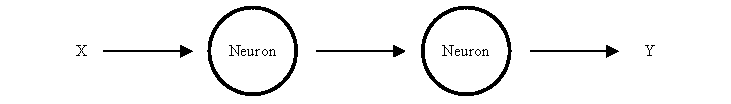
\includegraphics[width=0.9\textwidth]{../figs/Two_Neuron.drawio.pdf}
    \caption{Diagram of two neurons connected in series.}
    \label{fig:neuron}
\end{figure}

Let's say we have the following values of X and $\hat{Y}$ which correspond to the function y=$x^2 + 3x + 2$.:
\begin{table}[ht]
    \centering
    \begin{tabular}{|c|c|}
        \hline
        X & $\hat{Y}$ \\
        \hline
        0 & 2 \\
        \hline
        1 & 6 \\
        \hline
        2 & 12 \\
        \hline
    \end{tabular}
    \caption{Values of X and $\hat{Y}$}
    \label{tab:x_y_hat}
\end{table}

We know that the output of a single neuron is given by:
\[
    Y = W \cdot X + B
\]
We can think of this to be capable of representing the following function:
\[
    y = mx+c
\]

Obviously, a single neuron cannot represent the function $y=x^2 + 3x + 2$ as it is not a linear function. Two neurons, one after the other, may be a good starting point. However, they too are not capable of representing the function $y=x^2 + 3x + 2$.

Say the first neuron has weights $W_1$ and bias $B_1$, and the second neuron has weights $W_2$ and bias $B_2$. 

The output of the first neuron is given by:
\[
    Y_1 = W_1 \cdot X + B_1
\]
The output of the second neuron is given by:
\[
    Y_2 = W_2 \cdot Y_1 + B_2
\]
The output of the second neuron can be expressed as:
\[
    Y_2 = W_2 \cdot (W_1 \cdot X + b_1) + B_2
\]
Which simplifies to:
\[
    Y_2 = W_2 \cdot W_1 \cdot X + (W_2 \cdot B_1 + B_2)
\]

Unfortunately, this is still a linear function.

\section{Activation Function}
By the end of this lecture, we will read images of handwritten digits.

One key challenge to solve in our journey is to be able to represent more than just linear functions. We can do this by introducing an activation function. The activation function is a non-linear function that is applied to the output of the neuron before passing it to the next layer.

There are multiple activation functions. Here, they are generally represented with $f$. In our code example, I will use the tanh function as the activation function. The tanh function is defined as:
\[
    \text{tanh}(x) = \frac{e^x - e^{-x}}{e^x + e^{-x}}
\]
Which looks like this:

\begin{center}
    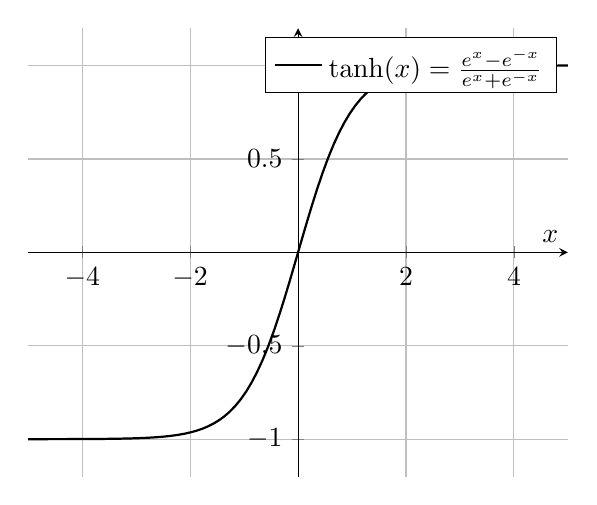
\begin{tikzpicture}
        \begin{axis}[
          axis lines = center,
          xlabel = $x$,
          ylabel = {tanh$(x)$},
          grid = both,
          xmin=-5, xmax=5,
          ymin=-1.2, ymax=1.2,
        ]
          \addplot[
            domain=-5:5,
            samples=100,
            color=black,
            thick,
          ]
          {tanh(x)}; % function to plot
          \addlegendentry{tanh$(x) = \frac{e^x - e^{-x}}{e^x + e^{-x}}$}
        \end{axis}
    \end{tikzpicture}
\end{center}

A neuron with an activation function can be represented as:
\[
    Y = \text{tanh}(W \cdot X + B)
\]

Now, we can represent non-linear and complex functions.
\subsection{Complex Problems as Complex Mathematical Functions}
Right now, it would be important for you to understand that almost any problem, something as challenging as reading handwritten digits, can be represented as a complex mathematical function. Only its coefficients are to be known. Often, these are matrix functions. By the end of this lecture, we will represent the function that can read handwritten digits. Usually, The more complex the function, the more neurons we need to represent it.

\section{Multi-Input Neuron}
\subsection{Biological Neurons}
\begin{figure}[ht]
    \centering
    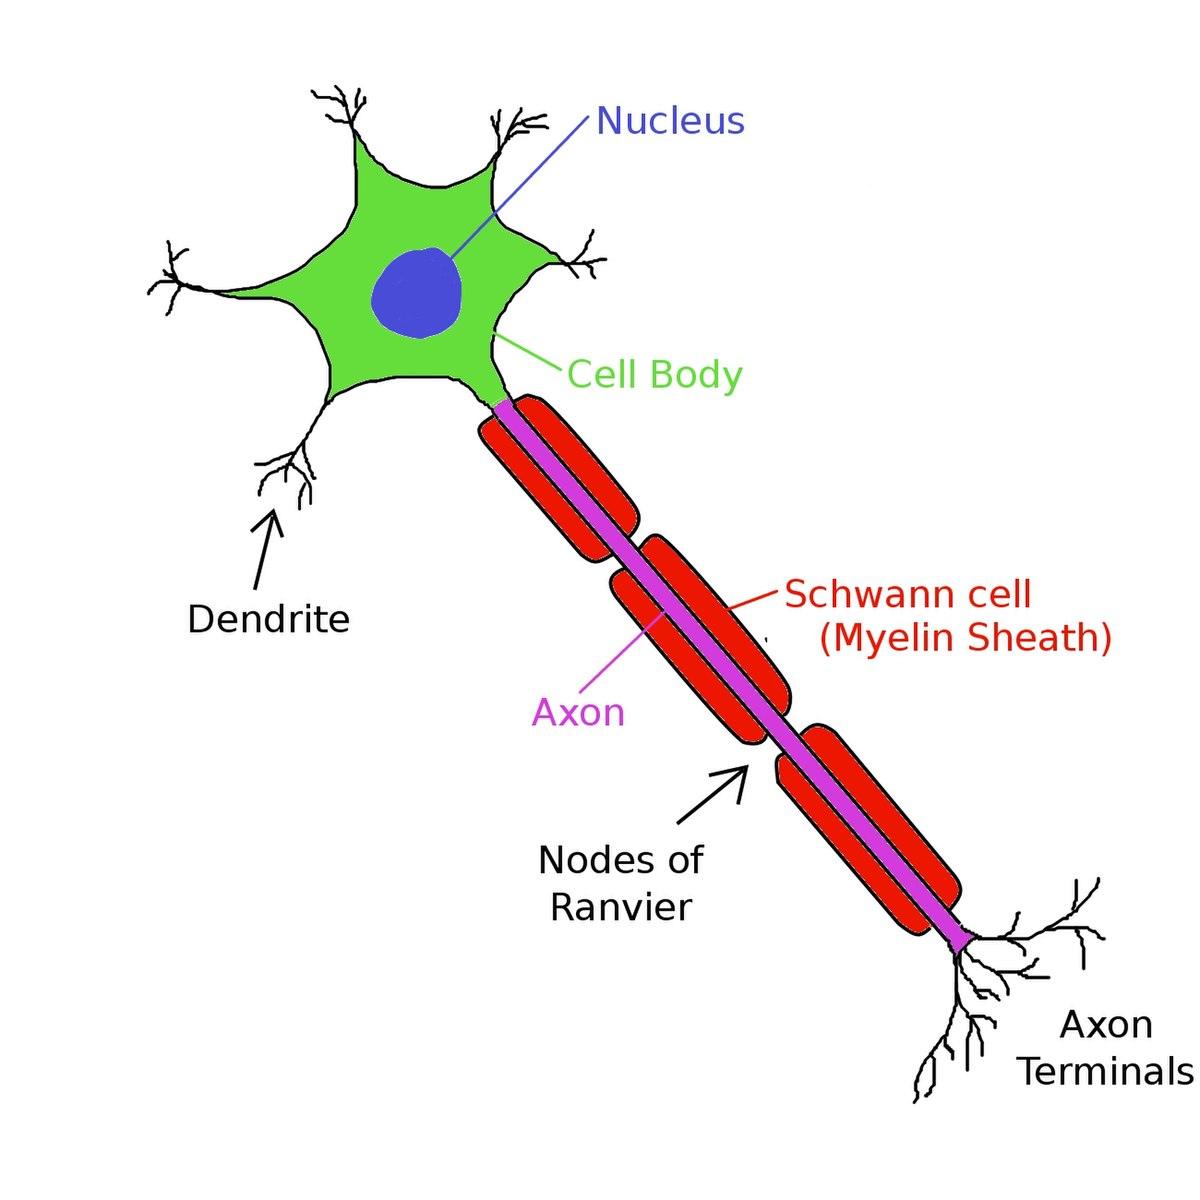
\includegraphics[width=0.55\textwidth]{../figs/Neuron_Diagram.jpg}
    \caption{Biological Neurons.}
    \label{fig:biulogical_neurons}
\end{figure}
A biological neuron is connected to multiple neurons. The distance between two neurons is variable. If the distance is small, the signal is strong. If the distance is large, the signal is weak. The signal is passed from one neuron to another through synapses. The synapse can be thought of as a weight. The synapse can be thought of as a weight. The synapse can be thought of as a weight. The synapse can be thought of as a weight.

Therefore, a true neuron takes inputs from multiple sources and has seperate weights for each. Additionally, a neuron has a single bias and a single output.
\subsection{Mathematical Representation}
\begin{figure}[ht]
    \centering
    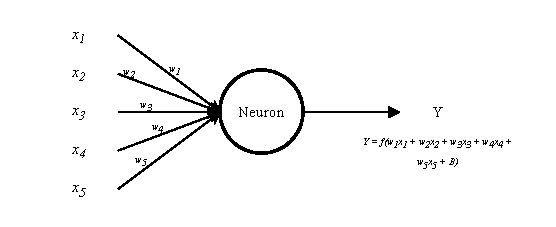
\includegraphics[width=0.9\textwidth]{../figs/Multi_input_neuron.drawio.pdf}
    \caption{Neuron capable of taking multiple inputs.}
    \label{fig:multiple_input_neuron}
\end{figure}
Say we are trying to build a neuron that adds three numbers, $x_1$, $x_2$, $x_3$. 
Let the set of inputs be a matrix X:
\[
    X = \begin{bmatrix}
        x_1\ \   x_2\ \   x_3
    \end{bmatrix}
\]

Let the set of weights be a matrix W:
\[
    W = \begin{bmatrix}
        w_1 \\   w_2 \\   w_3
    \end{bmatrix}
\]
\indent The output of the neuron is given by where @ is the matrix multiplication operator:
\[
Y = f(w_1 \cdot x_1 + w_2 \cdot x_2 + w_3 \cdot x_3 + B)
\]

We can represent this as a matrix multiplication:
\[
Y = f(X @ W + B)
\]
W is a 3x1 matrix and X is a 1x3 matrix. The result of the multiplication is a 1x1 matrix. The bias is added to the result of the multiplication.
\[
Y_{pre-activation} = \begin{bmatrix}
    w_1 \cdot x_1 + w_2 \cdot x_2 + w_3 \cdot x_3 
\end{bmatrix} 
+ 
\begin{bmatrix}
    B \\
\end{bmatrix}
\]

\[
Y = f(Y_{pre-activation})
\]

Additionally, if we had 5 training samples, each with 3 numbers to add, we can represent X as:
\[
    X = \begin{bmatrix}
        x_{11} & x_{12} & x_{13} \\
        x_{21} & x_{22} & x_{23} \\
        x_{31} & x_{32} & x_{33} \\
        x_{41} & x_{42} & x_{43} \\
        x_{51} & x_{52} & x_{53}
    \end{bmatrix}
\]

Doing the previous matrix multiplication of a 3x1 matrix with a 5x3 matrix, we get a 5x1 matrix. The bias belongs to the neuron, and the same bias is added to each element of the result.

\[
Y = X@W + B
\]

\[
Y_{pre-activation} = \begin{bmatrix}
    w_1 \cdot x_{11} + w_2 \cdot x_{12} + w_3 \cdot x_{13} \\
    w_1 \cdot x_{21} + w_2 \cdot x_{22} + w_3 \cdot x_{23} \\
    w_1 \cdot x_{31} + w_2 \cdot x_{32} + w_3 \cdot x_{33} \\
    w_1 \cdot x_{41} + w_2 \cdot x_{42} + w_3 \cdot x_{43} \\
    w_1 \cdot x_{51} + w_2 \cdot x_{52} + w_3 \cdot x_{53}
\end{bmatrix}
+
\begin{bmatrix}
    B \\
    B \\
    B \\
    B \\
    B
\end{bmatrix}
\]

\[
Y = f(Y_{pre-activation})
\]
We find that this is equivalent as calculating Y for each sample seperately. With this method, we were able to compute the output of 5 training samples all at once, with a single multiplication. Additionally, matrix multiplications are very efficient on GPUs. This is why we've been representing neurons with matrices.

\section{Dense Neural Network}
\subsection{Single Layer Network}
While reading handwritten digits, we will take a 28x28 image. It will have 784 pixels. Therefore, there are 784 inputs, also called "input neurons". (They aren't actually neurons.)

We have to predict if the image has one of 10 possible digits. Because our non linear function will compress inputs from 0 to 1, we can not represent outputs from 0 to 9 using a single neuron. Therefore, we have multiple output neurons. Each output neuron corresponds to a digit. Ideally, the output neuron will be 1 if the digit is present, and 0 if it is not.

In practice, the output neurons will have numbers from 0 to 1. The output neuron with the highest value will be the predicted digit. For example, if the output neurons are [0.1, 0.2, 0.3, 0.4, 0.5, 0.6, 0.7, 0.8, 0.9, 1], the predicted digit is 9 as the 9th neuron has the highest probability. The two neurons side by side form a 'layer'.

Additionally, instead of using tanh for our output neurons, we will use the softmax function. The softmax function is defined as:
\[
    \text{softmax}(x_i) = \frac{e^{x_i}}{\sum_{j=1}^{n} e^{x_j}}
\]
Where $x_i$ is the output of the neuron, and $n$ is the number of output neurons. The softmax function will ensure that the output neurons are between 0 and 1, and that they sum to 1.
The softmax function is used to convert the output of the neuron into a probability distribution. This is important because we want to predict the digit with the highest probability. Though tanh will also put numbers between 0 and 1, it will not ensure that they sum to 1. 

\textbf{Example:} Let's take a simpler example of 5 inputs and 2 possible outputs.
\begin{figure}[ht]
    \centering
    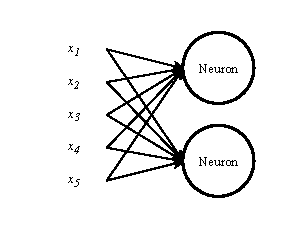
\includegraphics[width=0.55\textwidth]{../figs/Single layer DNN.drawio.pdf}
    \caption{A single layer neural network.}
    \label{fig:single_layer_dnn}
\end{figure}

Say we are training on 3 examples:
\[
X = \begin{bmatrix}
    x_{11} & x_{12} & x_{13} & x_{14} & x_{15} \\
    x_{21} & x_{22} & x_{23} & x_{24} & x_{25} \\
    x_{31} & x_{32} & x_{33} & x_{34} & x_{35}
\end{bmatrix}
\]

$W_1$ corresponds to the weights for the first neuron and $W_2$ corresponds to the weights for the second neuron. 
\[
W_1 = \begin{bmatrix}
    w_{11} \\ w_{12} \\ w_{13} \\ w_{14} \\ w_{15}
\end{bmatrix}
\]

\[
W_2 = \begin{bmatrix}
    w_{21} \\ w_{22} \\ w_{23} \\ w_{24} \\ w_{25}
\end{bmatrix}
\]
The output of the first neuron is given by:
\[
    Y_{1,\ pre-activation} =  X @ W_1 + B_1 \\
\]
\[
    Y_{1,\ pre-activation} = \begin{bmatrix}
        w_{11} \cdot x_{11} + w_{12} \cdot x_{12} + w_{13} \cdot x_{13} + w_{14} \cdot x_{14} + w_{15} \cdot x_{15} \\
        w_{11} \cdot x_{21} + w_{12} \cdot x_{22} + w_{13} \cdot x_{23} + w_{14} \cdot x_{24} + w_{15} \cdot x_{25} \\
        w_{11} \cdot x_{31} + w_{12} \cdot x_{32} + w_{13} \cdot x_{33} + w_{14} \cdot x_{34} + w_{15} \cdot x_{35}
    \end{bmatrix}
    + \begin{bmatrix}
        B_1 \\ 
        B_1 \\
        B_1
    \end{bmatrix}
\]

\indent The output of the second neuron is given by:
\[
Y_{2,\ pre-activation} =  X @ W_2 + B_2 \\
\]
\[
Y_{2,\ pre-activation} = \begin{bmatrix}
    w_{21} \cdot x_{11} + w_{22} \cdot x_{12} + w_{23} \cdot x_{13} + w_{24} \cdot x_{14} + w_{25} \cdot x_{15} \\
    w_{21} \cdot x_{21} + w_{22} \cdot x_{22} + w_{23} \cdot x_{23} + w_{24} \cdot x_{24} + w_{25} \cdot x_{25} \\
    w_{21} \cdot x_{31} + w_{22} \cdot x_{32} + w_{23} \cdot x_{33} + w_{24} \cdot x_{34} + w_{25} \cdot x_{35}
\end{bmatrix}
+ \begin{bmatrix}
    B_2 \\
    B_2 \\
    B_2
\end{bmatrix}
\]

We can write the final output of the layer like this:
\[
    Y_1 = f(Y_{1,\ pre-activation})
\] 
\[
    Y_2 = f(Y_{2,\ pre-activation})
\]
\[
    Y = \begin{bmatrix}
        Y_1 & Y_2
    \end{bmatrix}
\]

Alternatively:
\[
Y_{pre-activation} = \begin{bmatrix}
    Y_{1,\ pre-activation} & Y_{2,\ pre-activation}
\end{bmatrix}
\]
\[
Y_{pre-activation} = \begin{bmatrix}
    w_{11}x_{11} + w_{12}x_{12} + \cdots + w_{15}x_{15} + B_1  & w_{21}x_{11} + w_{22}x_{12} + \cdots + w_{25}x_{15} + B_2 \\
    w_{11}x_{21} + w_{12}x_{22} + \cdots + w_{15}x_{25} + B_1  & w_{21}x_{21} + w_{22}x_{22} + \cdots + w_{25}x_{25} + B_2\\
    w_{11}x_{31} + w_{12}x_{32} + \cdots + w_{15}x_{35} + B_1  & w_{21}x_{31} + w_{22}x_{32} + \cdots + w_{25}x_{35} + B_2
\end{bmatrix}
\]

\[
Y = f(Y_{pre-activation})
\]

We can do something more efficient, however.
If we write:
\[
W = \begin{bmatrix}
    W_1 & W_2
\end{bmatrix}
\]
\[
W = \begin{bmatrix}
    w_{11} & w_{21} \\
    w_{12} & w_{22} \\
    w_{13} & w_{23} \\
    w_{14} & w_{24} \\
    w_{15} & w_{25}
\end{bmatrix}
\]
And,
\[
B = \begin{bmatrix}
    B_1 & B_2 \\
    B_1 & B_2 \\
    B_1 & B_2 \\
\end{bmatrix}
\]
Now, if we write:
\[
Y_{pre-activation} = X @ W + B
\]
We get:
\[
Y_{pre-activation} = \begin{bmatrix}
    w_{11}x_{11} + w_{12}x_{12}+ \cdots + w_{15}x_{15} + B_1  & w_{21}x_{11} + w_{22}x_{12} + \cdots + w_{25}x_{15} + B_2 \\
    w_{11}x_{21} + w_{12}x_{22} + \cdots + w_{15}x_{25} + B_1  & w_{21}x_{21} + w_{22}x_{22} + \cdots + w_{25}x_{25} + B_2 \\
    w_{11}x_{31} + w_{12}x_{32} + \cdots + w_{15}x_{35} + B_1  & w_{21}x_{31} + w_{22}x_{32} + \cdots + w_{25}x_{35} + B_2 
\end{bmatrix}
\]
This is equivalent to the previous two matrix multiplication. What we have found is that not only can we represent all the computation in a neuron with a single matrix multiply follow by an addition, but that we can also represent an entire layer with the same computation. Of course, this single multiplication will take longer to compute.

\subsection{Inferences}
Now that the concepts behind the following have been understood, I would recommend remembering these points:
\begin{itemize}
    \item We have found that an input layer is a row matrix for a single training example of shape (1) x (number of inputs).
    \item The number of training examples is called the batch size.
    \item For multiple training examples, the input layer is a matrix with each row being a training example (batch size) x (number of inputs).
    \item The weights of the neuron are a column matrix of shape (number of inputs) x (1).
    \item The output of the neuron is a column matrix of shape (batch size) x (1).
    \item The weights of a layer are of shape (number of inputs) x (number of neurons).
    \item The output of a layer has the shape (batch size) x (number of neurons).  
    \item The bias of a layer is a matrix of shape (batch size) x (number of neurons) where all rows have the same values.
\end{itemize}
\newpage

\subsection{Three Layer Example}
For complex problems like reading handwritten digits, we need to stack multiple neuron layers together, each with multiple neurons. 
\begin{figure}[ht]
    \centering
    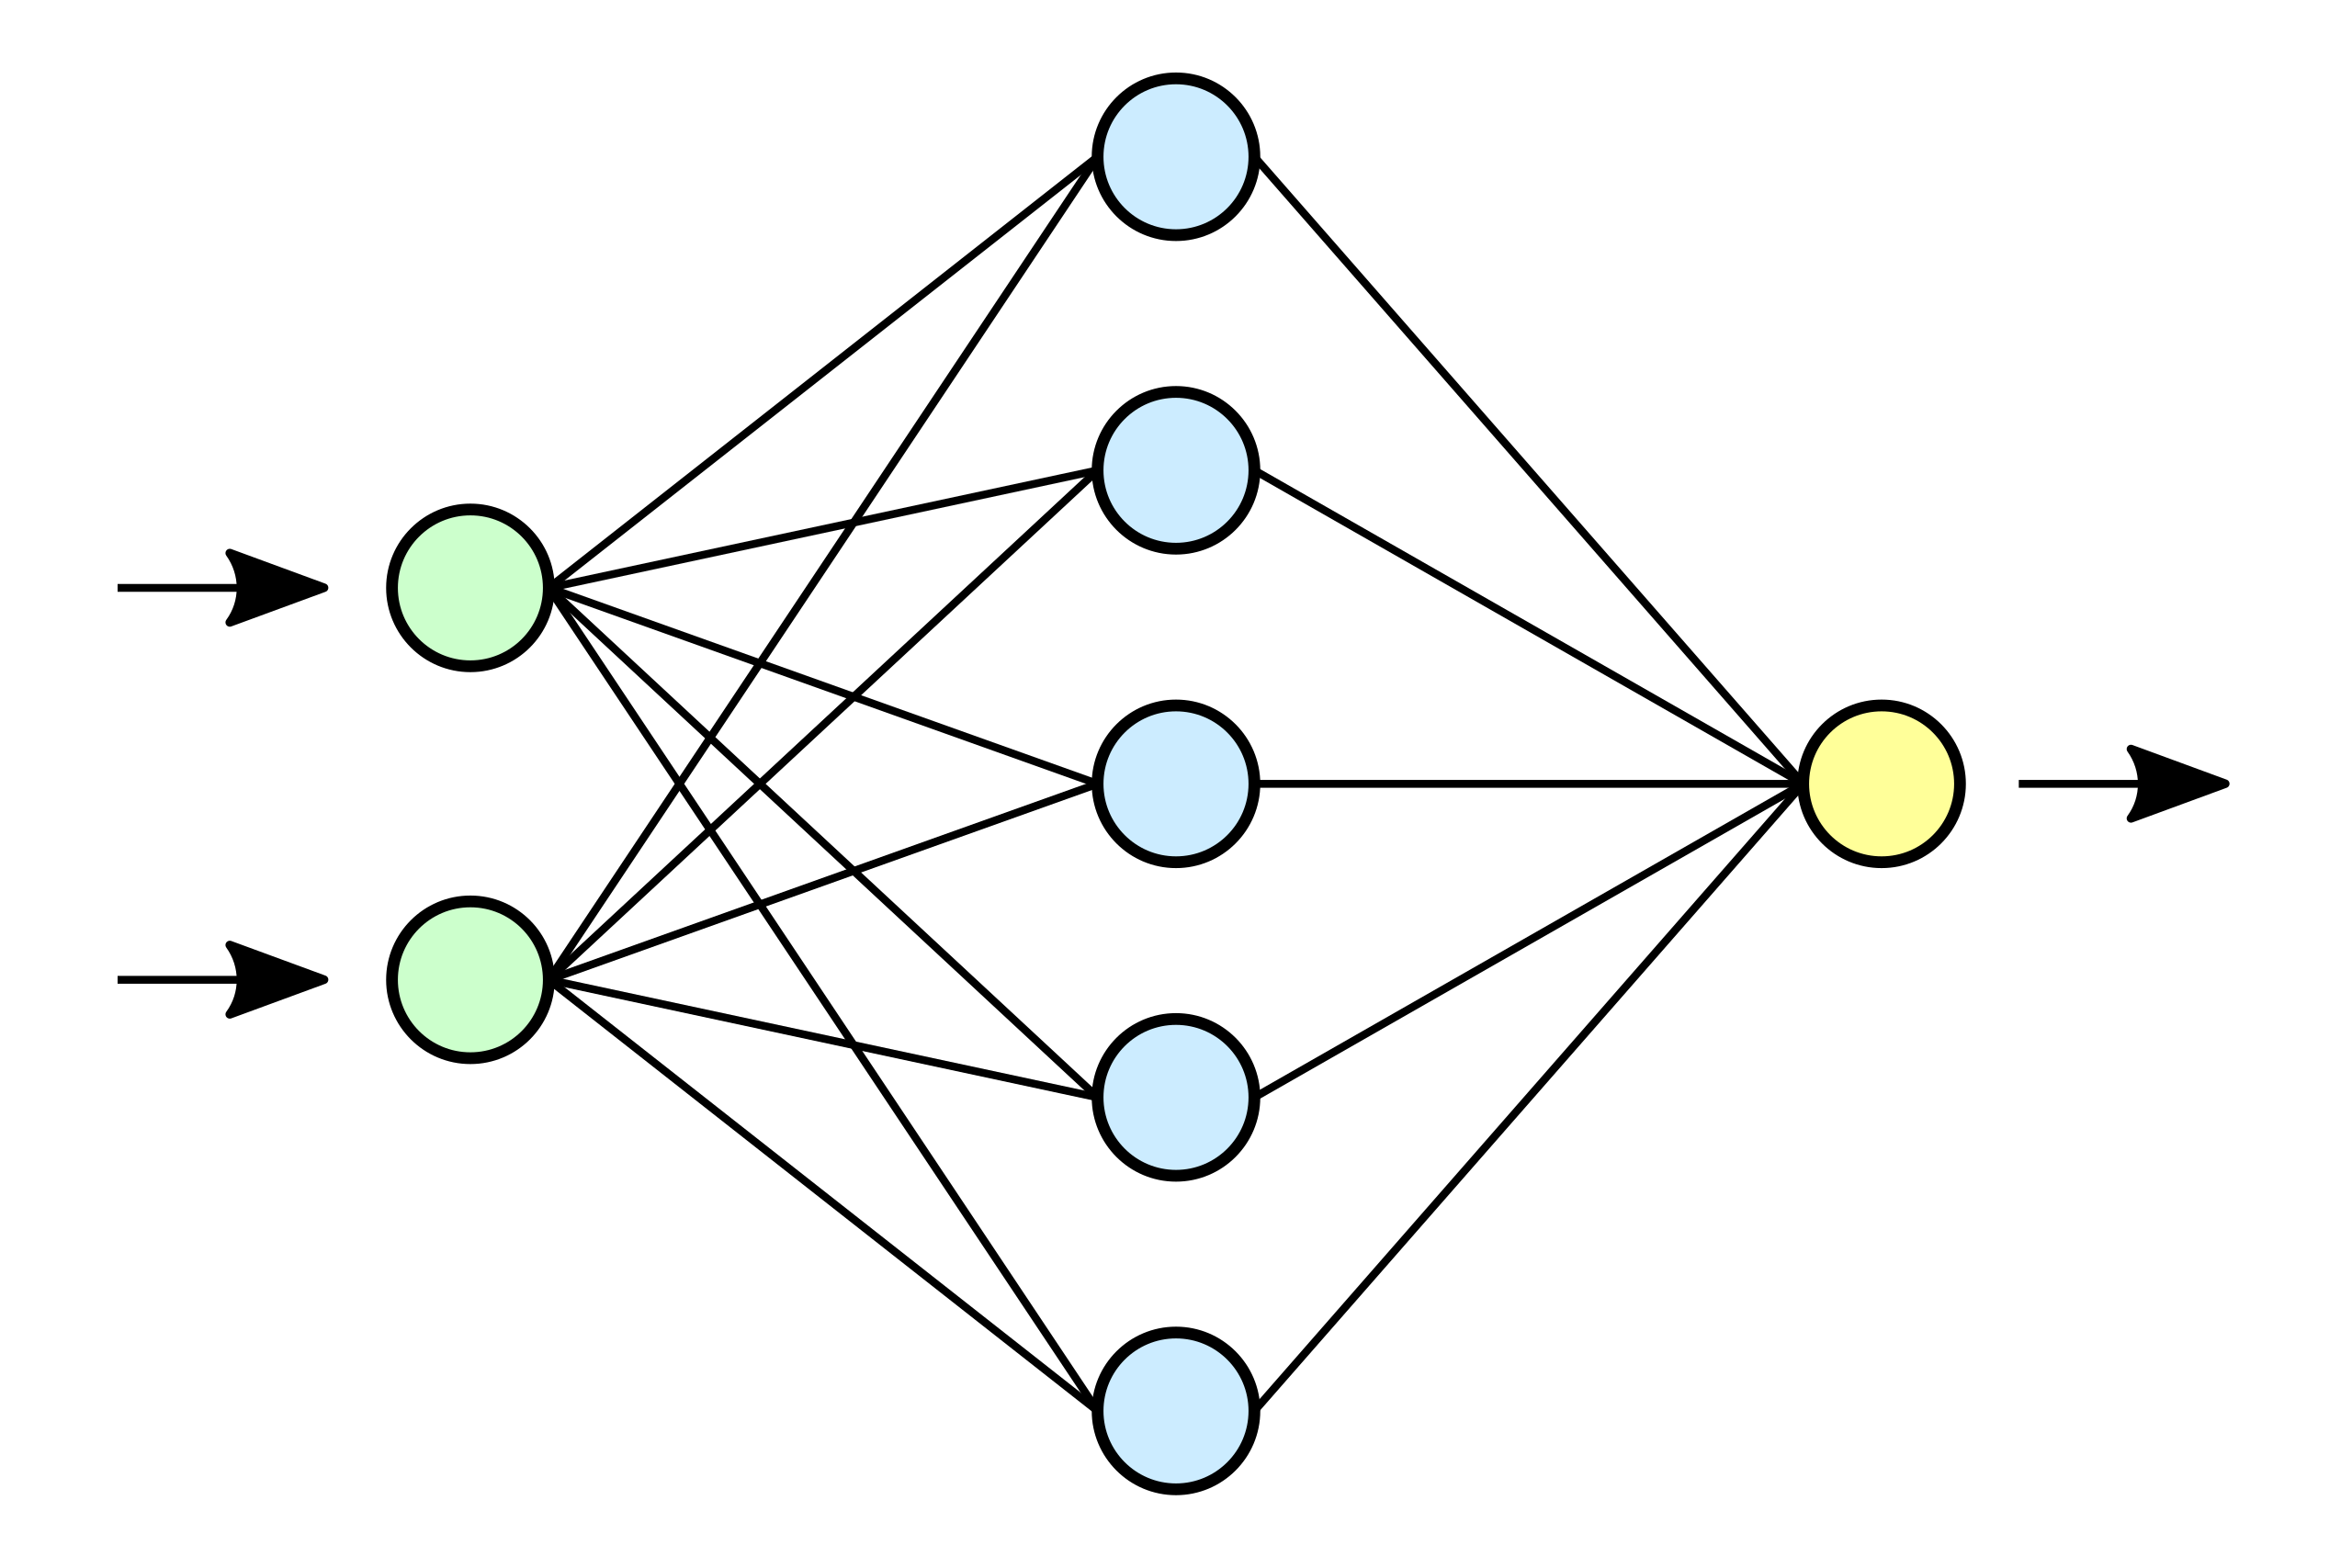
\includegraphics[width=0.7\textwidth]{../figs/Neural_network.svg.png}
    \caption{A Dense Neural Network.}
    \label{fig:DNN}
\end{figure}

Though I had shown inputs with $x_1$, $x_2$, $x_3$ in previous diagrams, it is convention in diagrams to show the inputs as neurons as well (though they are not). The inputs are represented as neurons in the diagram below. The first layer is the input layer, the second layer is the hidden layer, and the third layer is the output layer. The input layer has 2 neurons, the hidden layer has 5 neurons, and the output layer has 1 neuron.

$W_1$ corresponds to the weights for the hidden layer, and $W_2$ corresponds to the weights for the output layer. The biases are represented as $B_1$ and $B_2$. $Y_1$ and $Y_2$ are the outputs of the hidden layer and output layer respectively. 
\begin{itemize}
    \item X is of shape (batch size) x (2).
    \item $W_1$ is of shape (2) x (5).
    \item $B_1$ is of shape (batch size) x (5).
    \item $Y_1 = f(X @ W_1 + B_1)$ is of shape (batch size) x (5).
    \item $W_2$ is of shape (5) x (1).
    \item $B_2$ is of shape (batch size) x (1).
    \item $Y_2 = f(Y_1 @ W_2 + B_2)$ is of shape (batch size) x (1).
    \item $Y_2$ is the final output of the network.
\end{itemize}

\section{Practical Problems and Concluding Remarks}
\begin{itemize}
    \item We have only discussed the forward pass of this network as of yet. The backward pass will be manually calculated in AI 1.4.
    \item Dense Neural Neworks are mathematially capable of solving very complex problems. However, in practice, they struggle in finding the best solution. They get stuck at local minimas. 
    \item These models, along with most models in modern AI, are trained once on known samples, and then used for inference. Unfortunately, it is not possible for these models to learn on their own, without many labels like humans do. Neither are they capable of learning while in inference and updating their learnings on the fly. There are many other major limitations of the current way AI is done, which we will look at later.
    \item Look at AI-12.ipynb to implement a model that can read handwritten digits. 
\end{itemize}

\end{document}